\problemname{Problem 5 - Wreck Tangles}

Professor Plum occasionally teaches Operating Systems, and this problem reminds him of the opposite of deadlock.

Bad news. Four strings all pulled up to a four-way stop at exactly the same time. None yielded, and all four mutually collided with each other and are in a pile-up. Interestingly, they overlap each other only where they have common letters. For example, suppose dragon is the north string, antelope the east, eagle the south, and badger the west. These four might pile up in several ways:

\begin{figure}[h]
\begin{center}
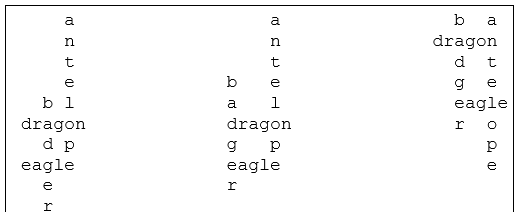
\includegraphics{problem5words.png} 
\end{center}
\end{figure}

Given any four strings, in how many possible arrangements may they pile up? The four strings must enclose at least one empty square. (The pile-ups above enclose $1$, $3$, and $4$ empty squares, respectively.)

\section*{Input}
The input consists of a number of cases followed by a sequence of four strings for each test case. The order of the strings is north-east-south-west.

\section*{Output}
For each case, print a case label and the number of possible pile-ups. For the above input, the output is:
